\let\negmedspace\undefined
\let\negthickspace\undefined
\documentclass[journal]{IEEEtran}
\usepackage[a5paper, margin=10mm, onecolumn]{geometry}
%\usepackage{lmodern} 
\usepackage{tfrupee} 

\setlength{\headheight}{1cm} 
\setlength{\headsep}{0mm}     

\usepackage{gvv-book}
\usepackage{gvv}
\usepackage{cite}
\usepackage{amsmath,amssymb,amsfonts,amsthm}
\usepackage{algorithmic}
\usepackage{graphicx}
\usepackage{textcomp}
\usepackage{xcolor}
\usepackage{txfonts}
\usepackage{listings}
\usepackage{enumitem}
\usepackage{mathtools}
\usepackage{gensymb}
\usepackage{comment}
\usepackage[breaklinks=true]{hyperref}
\usepackage{tkz-euclide} 
\usepackage{listings}                                        
\def\inputGnumericTable{} 
\usepackage[latin1]{inputenc}                                
\usepackage{color}                                            
\usepackage{array}                                            
\usepackage{longtable}                                       
\usepackage{calc}                                             
\usepackage{multirow}                                         
\usepackage{hhline}                                           
\usepackage{ifthen}                                           
\usepackage{lscape}

\begin{document}

\bibliographystyle{IEEEtran}
\vspace{3cm}

\title{2.2.16}
\author{AI25BTECH11023 - Pratik R}
{\let\newpage\relax\maketitle}

\renewcommand{\thefigure}{\theenumi}
\renewcommand{\thetable}{\theenumi}
\setlength{\intextsep}{10pt} 


\numberwithin{equation}{enumi}
\numberwithin{figure}{enumi}
\renewcommand{\thetable}{\theenumi}

\textbf{Question: }\\
The angle between the planes
$$
\vec{r} \cdot (2\hat{i}-3\hat{j}+\hat{k})=1 \text{ and } 
$$
$$
\vec{r} \cdot(\hat{i}-\hat{j})=4
$$
\textbf{Solution: } \\
Let $P_1$ and $P_2$ are the planes given respectively. \\
The normal vector of the planes, say $n_1$ and $n_2$ are:
\begin{align}
    \vec{n_1}= \myvec{2 \\ -3 \\ 1} \\
    \vec{n_1}= \myvec{1 \\ -1 \\ 0}
\end{align}

Thus, the cosine of the angle between the two is


\begin{align}
   \cos \theta = \frac{\vec{n_1} \cdot \vec{n_1}}{|n_1||n_2|}  
\end{align}
\begin{align}
    = \frac{5}{\sqrt{14}\times\sqrt{2}} = \frac{5}{\sqrt{28}}
\end{align}
\begin{align}
    \implies \theta = \cos ^{-1}\frac{5}{\sqrt{28}}
\end{align}
where $\theta$ is the acute angle between the planes.

\begin{figure}[H]
    \centering
    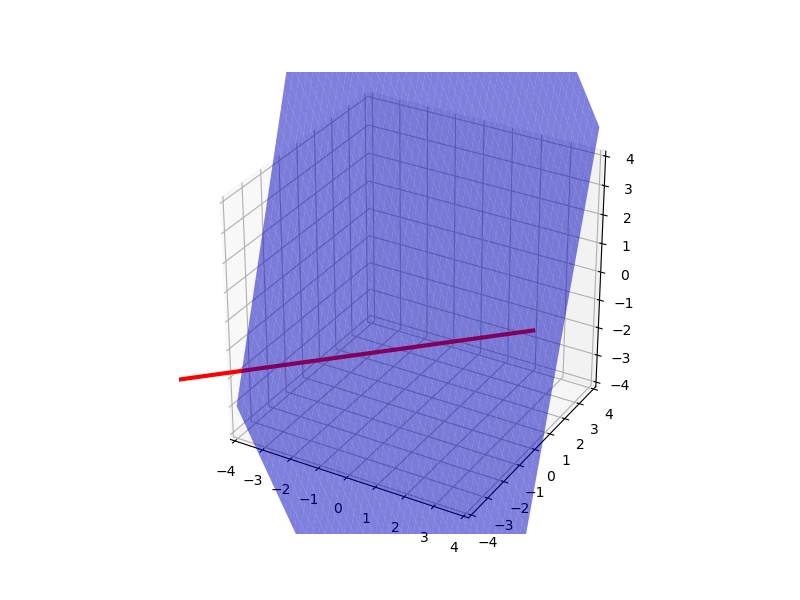
\includegraphics[width=0.7\columnwidth]{figs/fig.png}
    \caption*{}
\end{figure}


\end{document}
